\input{../YKY-preamble.tex}
\setmainfont[BoldFont=Alibaba_Sans_Regular.otf,ItalicFont=Alibaba_Sans_Light_Italic.otf]{Alibaba_Sans_Light.otf}
	
\usepackage[active,tightpage]{preview}		% for continuous page(s)
\renewcommand{\PreviewBorder}{0.5cm}
\renewcommand{\thempfootnote}{\arabic{mpfootnote}}

\usepackage[absolute,overlay]{textpos}		% for page number on upper left corner

\usepackage{color}
\usepackage{mathtools}
\usepackage[hyperfootnotes=false]{hyperref}

% \usepackage[backend=biber,style=numeric]{biblatex}
% \bibliography{../AGI-book}
% \renewcommand*{\bibfont}{\footnotesize}

\usetikzlibrary{shapes}
\usepackage[export]{adjustbox}				% ??
\usepackage{verbatim} % for comments
% \usepackage{newtxtext,newtxmath}	% Times New Roman font

% \numberwithin{equation}{subsection}

\newcommand{\underdash}[1]{%
	\tikz[baseline=(toUnderline.base)]{
		\node[inner sep=1pt,outer sep=10pt] (toUnderline) {#1};
		\draw[dashed] ([yshift=-0pt]toUnderline.south west) -- ([yshift=-0pt]toUnderline.south east);
	}%
}%


%\DeclareSymbolFont{symbolsC}{U}{txsyc}{m}{n}
%\DeclareMathSymbol{\strictif}{\mathrel}{symbolsC}{74}
\DeclareSymbolFont{AMSb}{U}{msb}{m}{n}
\DeclareSymbolFontAlphabet{\mathbb}{AMSb}
% \setmathfont{Latin Modern Math}
\DeclareMathOperator*{\argmin}{arg\,min}

% \usepackage[most]{tcolorbox}
\tcbset{on line, 
	boxsep=4pt, left=0pt,right=0pt,top=0pt,bottom=0pt,
	colframe=red,colback=pink,
	highlight math style={enhanced}
}
\newcommand{\atom}{\vcenter{\hbox{\tcbox{....}}}}

% \newcommand{\emp}[1]{{\color{violet}\textbf{#1}}}
\let\oldtextbf\textbf
\renewcommand{\textbf}[1]{\textcolor{blue}{\oldtextbf{#1}}}

\newcommand{\logic}[1]{{\color{violet}{\textit{#1}}}}
\newcommand*\smileFace{$\vcenter{\hbox{\includegraphics[scale=0.6]{../smiley.jpg}}}$}
\newcommand{\underconst}{\includegraphics[scale=0.5]{../2020/UnderConst.png}}
\newcommand{\KBsymbol}{\vcenter{\hbox{\includegraphics[scale=1]{../KB-symbol.png}}}}
\newcommand{\witness}{\scalebox{0.6}{$\blacksquare$}}
% \newcommand{\Heytingarrow}{\mathrel{-}\mathrel{\triangleright}}
% \providecommand\Heytingarrow{\relbar\joinrel\mathrel{\vcenter{\hbox{\scalebox{0.75}{$\rhd$}}}}}

\begin{document}

\begin{preview}

\cc{
\title{\vspace{-1.5cm} \bfseries\color{blue}{\Large 逻辑与深度学习的关系}}
}{
\title{\vspace{-1.5cm} \bfseries\color{blue}{\Large Comparison of Logic AI and Deep Learning}}
}

% \author{YKY} % Your name
\date{\vspace{-2cm}} % Date, can be changed to a custom date

\maketitle

\setcounter{section}{-1}

% (1) Circled page number on upper left corner
\begin{textblock*}{5cm}(2.1cm,2.3cm) % {block width} (coords) 
{\color{red}{\large \textcircled{\small 1}}}
\end{textblock*}

\begin{minipage}{\textwidth}
\setlength{\parskip}{0.4\baselineskip}

\cc{这是经典逻辑 AI 的最基本运作模式:
}{
This is the most basic mode of operation of classical logic AI:
}
\begin{equation}
\cc{  \vcenter{\hbox{
\includegraphics[scale=1]{LBAI-basic-config.png}}}     }{
      \vcenter{\hbox{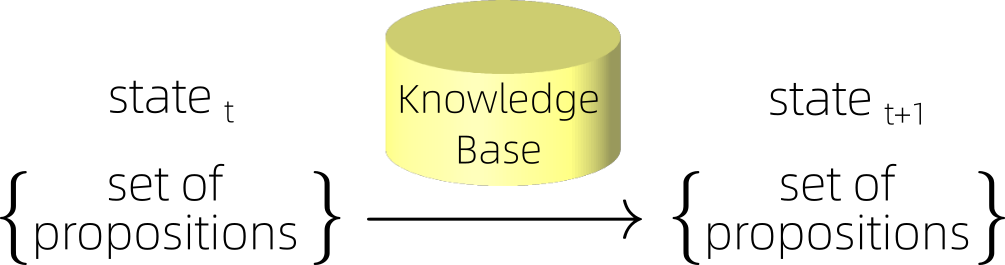
\includegraphics[scale=1]{LBAI-basic-config-en.png}}}  }
\end{equation}

\cc{它其实包含了两个算法:
}{
It actually contains two algorithms:
}
\begin{itemize}
	\item \textbf{matching} (unification): \\
\cc{	逻辑 rules 是包含变量的条件命题, \\
}{
Logical rules are conditional propositions involving variables, \\
}
\cc{	例如 \tab \logic{$\forall x. \mbox{是人}(x) \Rightarrow \mbox{会死}(x). $ }\\
}{
For example \tab \logic{$\forall x. \mbox{human}(x) \Rightarrow \mbox{mortal}(x). $ }\\
}
\cc{	Unification 判定一条 rule 是否可以 apply 到某逻辑命题上,\\
}{
Unification determines whether a rule can be applied to a logical proposition,\\
}
\cc{	例如:\logic{是人(苏格拉底)} 可以跟上式的左边 unify. \\
}{
For example: \logic{human(Socrates)} can unify the left side of the formula. \\
}
\cc{	Matching 的结果是得到一推 instantiated(特例化,即不包含变量)的命题。
}{
The result of Matching is to get a proposition that is instantiated (specialized, that is, does not contain variables).
}
	
	\item \textbf{forward- or backward-chaining} (resolution): \\
\cc{	由已知事实 推导出新结论,或反过来,判断某给定的新结论是否成立。 \\
}{
Deduce new conclusions from known facts, or conversely, judge whether a given new conclusion is established. \\
}
\cc{	例如:\logic{ 是人(苏格拉底) $\Rightarrow$ 会死(苏格拉底) $\;\; \wedge$ 是人(苏格拉底) } \\
}{
For example: \logic{human (Socrates) $\wedge \;$ human(Socrates) $\Rightarrow$ mortal(Socrates)} \\
}
\cc{	可以推出:\logic{会死(苏格拉底)}。
}{
It can be deduced: \logic{mortal (Socrates)}.
}
\end{itemize}

\cc{深度学习的特点,就是将
}{
The characteristics of deep learning are the
}
\begin{equation}
\mbox{\cc{状态}{state}}_t  \vdash \mbox{\cc{状态}{state}}_{t+1}
\end{equation}
\cc{的逻辑推导过程,通通纳入进去一个非常复杂的非线性函数(= 深度神经网络)里面。 这样做以后,上述的逻辑结构被
}{
The logical derivation process is all incorporated into a very complex nonlinear function (= deep neural network). After doing so, the above logical structure is
}
\cc{``mingled'' 在一起,以至于很难分辨了。 但也正是由于这种「大杂烩」,深度神经网络 将一套复杂的组合算法 压缩成数量不算太多的一层层的参数。 它同时可以做 learning 和 inference 这两个动作。 这种简单粗暴的方法,其实非常有效率,要超越它的速度并不容易!
}{
``mingled'' together so that it's hard to tell. But it is precisely because of this "hodgepodge" that the deep neural network compresses a set of complex combination algorithms into a small number of layer-by-layer parameters. It can do both learning and inference at the same time. This simple and crude method is actually very efficient, and it is not easy to surpass its speed!
}

\cc{我们知道(或推测)一个智能系统 应该具有 符号逻辑的结构。 这点知识可不可以用来 约束/加速 深度神经网络? 答案似乎是有可能的。 现时 state-of-the-art 处理 视觉的 CNN 和 处理文字的 BERT,它们都有内部结构, \textbf{而不是 fully-connected},而且 这内部结构 对应于 被处理的资料的结构。 因此我们有理由相信,逻辑结构 可以用来约束 深度神经网络的结构,达到加速。 
}{
We know (or speculate) that an intelligent system should have the structure of symbolic logic. Can this knowledge be used to constrain/accelerate deep neural networks? The answer seems to be possible. The current state-of-the-art CNN for vision and BERT for text both have an internal structure, \textbf{rather than fully-connected}, and this internal structure corresponds to the structure of the processed data. Therefore, we have reason to believe that the logical structure can be used to constrain the structure of the deep neural network to achieve acceleration.
}

\end{minipage}
\end{preview}

\begin{preview}
\begin{minipage}{\textwidth}
\setlength{\parskip}{0.4\baselineskip}

\begin{textblock*}{20cm}(2.1cm,2cm) % {block width} (coords) 
	{\color{red}{\large \textcircled{\small 2}}}
	\hspace{8cm}
	\color{blue}{\footnotesize \cc{逻辑与深度学习}{Logic and Deep Learning}}
\end{textblock*}
\vspace*{0.3cm} 

\cc{接下来我们详细一点看逻辑系统的结构:
}{
Next, let's look at the structure of the logical system in detail:
}

\cc{Knowledge Base 里面有很多 rules,系统要将这些 rules 逐一 match with 系统状态 (= working memory) 里面的命题:
}{
There are many rules in the Knowledge Base, and the system needs to match these rules one by one with the propositions in the system state (= working memory):
}
\begin{equation}
\vcenter{\hbox{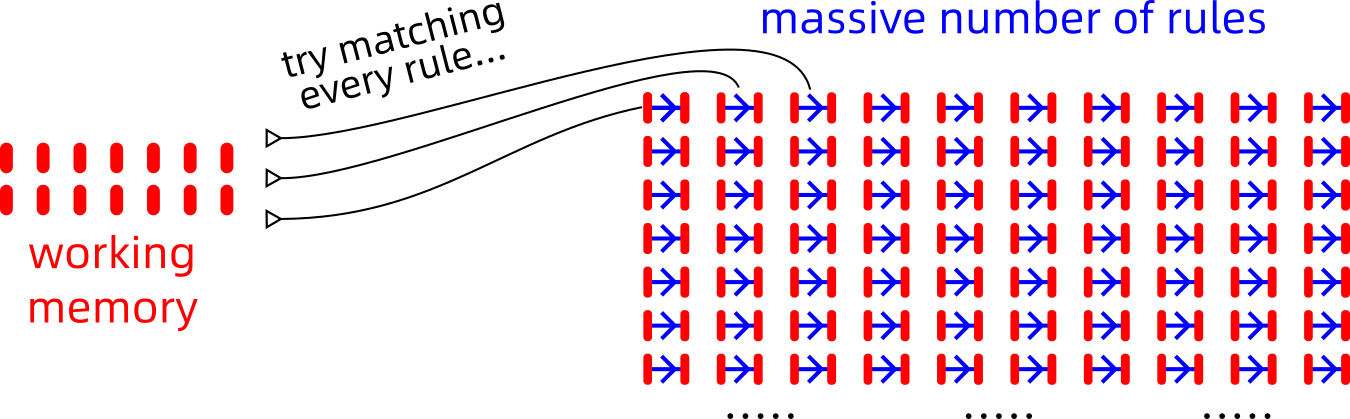
\includegraphics[scale=1]{rete-explained-1b.png}}}
\end{equation}
\cc{成功 matched 的 rules 可以导出新的结论,加进 working memory 的状态 里面。
}{
Successfully matched rules can derive new conclusions and add them to the state of working memory.
}

\cc{这个复杂的操作,完全被一个神经网络取代。 或者可以更抽象地说:
}{
This complex operation is completely replaced by a neural network. Or more abstractly:
}
\begin{equation}
\label{eqn:some-kind-of-memory}
\cc{ \vcenter{\hbox{
\includegraphics[scale=1]{some-kind-of-memory.png}}}    }{
     \vcenter{\hbox{
\includegraphics[scale=1]{some-kind-of-memory-en.png}}} }
\end{equation}

\cc{而以 Transformer 来说,它是一种 输入元 \textbf{之间} 的记忆体(这记忆就储存在 $Q, K, V$ 矩阵里),而它 \textbf{implicitly} 做到了 rules 的作用:
}{
For Transformer, it is a kind of memory between the input elements \textbf{between} (this memory is stored in the $Q, K, V$ matrices), and it \textbf{implicitly} achieves the role of rules:
}
\begin{equation}
\label{fig:self-attention-as-Rete}
\vcenter{\hbox{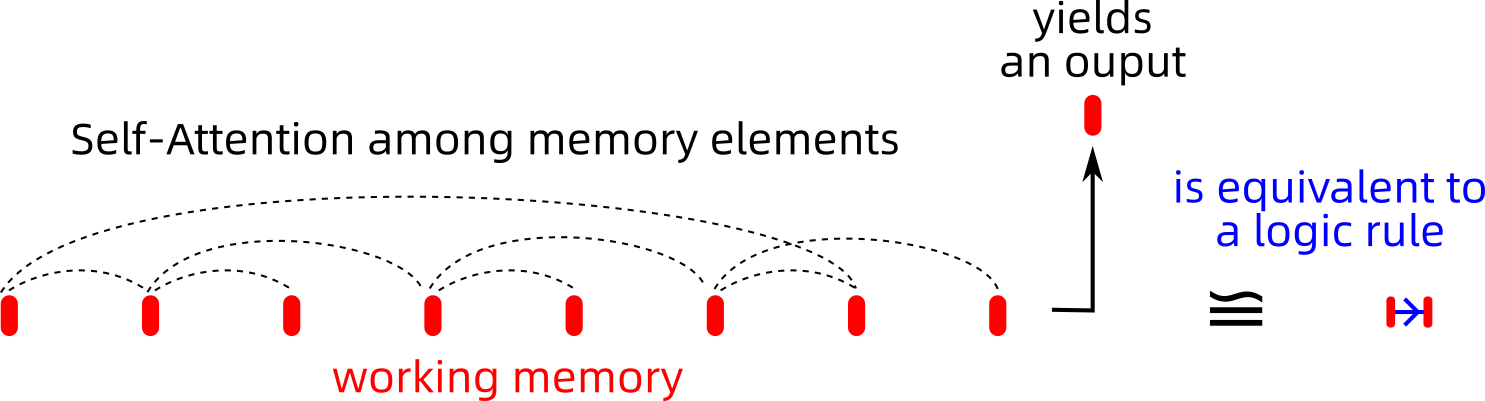
\includegraphics[scale=0.9]{rete-explained-3b.png}}}
\end{equation}
\cc{换句话说,Transformer 内部有某种(扭曲了的)逻辑 rules 的结构。 那么很自然的问题就是:能否发掘更多 逻辑/逻辑系统 的结构? 也就是说,公式 (\ref{eqn:some-kind-of-memory}) 可以有怎样的代数结构约束? 这个问题 可以参考 范畴逻辑 的理论,还有 经典 logic-based AI 系统的理论。
}{
In other words, there is some sort of (distorted) structure of logical rules inside the Transformer. The natural question then is: Can more structures of logic/logic systems be discovered? That is, what kind of algebraic structure constraints can the formula (\ref{eqn:some-kind-of-memory}) have? For this question, you can refer to the theory of category logic and the theory of classic logic-based AI systems.
}

\end{minipage}
\end{preview}

\begin{preview}
\begin{minipage}{\textwidth}
	
\setlength{\parskip}{0.4\baselineskip}
\begin{textblock*}{20cm}(2.1cm,2cm) % {block width} (coords) 
	{\color{red}{\large \textcircled{\small 3}}}
	\hspace{8cm}
	\color{blue}{\footnotesize \cc{逻辑与深度学习}{Logic and Deep Learning}}
\end{textblock*}
\vspace*{0.3cm} 

\cc{我们希望 勾画出公式 (\ref{eqn:some-kind-of-memory}) 需要具备的代数约束,但暂时先用文字描述比较容易:
}{
We wish to sketch out the algebraic constraints that the formula (\ref{eqn:some-kind-of-memory}) needs to have, but it is easier to describe in words for now:
}
\begin{itemize}
	\cc{	\item 状态是 \textbf{颗粒化} 的,它是某集合的元素,元素之间可交换,也就是 Transformer 的 equivariance. (注意: Transformer 有 equivariance,但 equivariance 未必一定要用 Transformer 实现)
	}{
		\item The state is \textbf{granularized}, it is an element of a certain set, and the elements can be exchanged, that is, the equivariance of Transformer. (Note: Transformer has equivariance, but equivariance does not necessarily have to be realized by Transformer)
	}
	
	\cc{	\item \textbf{深度结构}:例如多层网络,每层是函数的复合 (composition). Transformer 也用了深度结构。
	}{
		\item \textbf{Deep structure}: For example, a multi-layer network, each layer is a composition of functions. Transformer also uses a deep structure.
	}
	
	\cc{	\item 逻辑 包括了 \textbf{命题}层次 和 \textbf{命题内部}层次 的 颗粒化。 后者是\textbf{谓词} (predicate) 逻辑的结构,例如: \logic{loves( John, Mary )},也可以简单地将它视为 \textbf{代数元}之间的\textbf{乘积},例如: \logic{John \bullet\  loves \bullet\   Mary}, 后者也叫做 ``word''.  (不同类别的代数元之间不一定容许乘积,因此有 groupoid 的概念,但暂时来说这细节不重要。) 现时重点是如何将 这两层的 颗粒化 结构 施加到深度神经网络上。 
	}{
		\item Logic includes granularity at the \textbf{proposition} level and at the \textbf{inside a proposition} level. The latter is the structure of \textbf{predicate} (predicate) logic, for example: \logic{loves( John, Mary )}, it can also be simply regarded as the \textbf{product} between \textbf{algebraic elements} , for example: \logic{John \bullet\ loves \bullet\ Mary}, the latter is also called ``word''. The details are not important.) The focus now is on how to apply the granular structure of these two layers to deep neural networks.
	}
	
	\cc{	\item 逻辑推导 每步只产生\textbf{一个}新的结论(或其概率分布),然后这个新的结论,再加入到旧的状态中,作为一个命题集合的元素,而旧状态也要 \textbf{遗忘} 一些命题,否则需要无限记忆。 这跟 Transformer 每次输出\textbf{一列}的 tokens 有点不同(虽然我们不太肯定 Transformer tokens 究竟对应于 命题 还是 谓词/原子概念)。 
	}{
		\item Each step of logical derivation only produces \textbf{a} new conclusion (or its probability distribution), and then this new conclusion is added to the old state as an element of a proposition set, and the old state also needs to be \ textbf{forget} Some propositions, otherwise infinite memory is required. This is a bit different from Transformer outputting \textbf{column} tokens at a time (although we are not sure whether Transformer tokens correspond to propositions or predicate/atomic concepts).
	}
	
	\cc{	\item 逻辑 rule 通常只跟某几个前提有关,其它前提是\textbf{无关}的,例如: \logic{眼睛好看 $\wedge$ 鼻子好看 $\wedge$ 嘴巴好看 $\Rightarrow$ 帅},跟 \logic{有钱} 或 \logic{穷} 无关。 Transformer 的 \textbf{softmax} 结构似乎也可以排除一些无关的 tokens 的影响。
	}{
		\item logical rule is usually only related to some premises, other premises are \textbf{irrelevant}, for example: \logic{eyes beautiful $\wedge$ nose beautiful $\wedge$ mouth beautiful $\Rightarrow$ handsome}, where \logic{rich} or \logic{poor} is irrelevant. Transformer's \textbf{softmax} structure also seems to be able to exclude the influence of some irrelevant tokens.
	}
	
	\cc{	\item (可能还有其他的结构特征.....)
	}{
		\item (and possibly other structural features.....)
	}
\end{itemize}

\end{minipage}
\end{preview}

\begin{preview}
\begin{minipage}{\textwidth}

\setlength{\parskip}{0.4\baselineskip}
\begin{textblock*}{20cm}(2.1cm,2cm) % {block width} (coords) 
	{\color{red}{\large \textcircled{\small 4}}}
	\hspace{8cm}
	\color{blue}{\footnotesize \cc{逻辑与深度学习}{Logic and Deep Learning}}
\end{textblock*}
\vspace*{0.3cm} 

\cc{根据我的理论,理想的逻辑形式是这样的(各种元素的个数纯粹示意):
}{
According to my theory, the ideal logical form is this (the number of various elements is purely indicative):
}
\begin{equation}
\label{fig:logic-symmetry-predicate-level}
\vcenter{\hbox{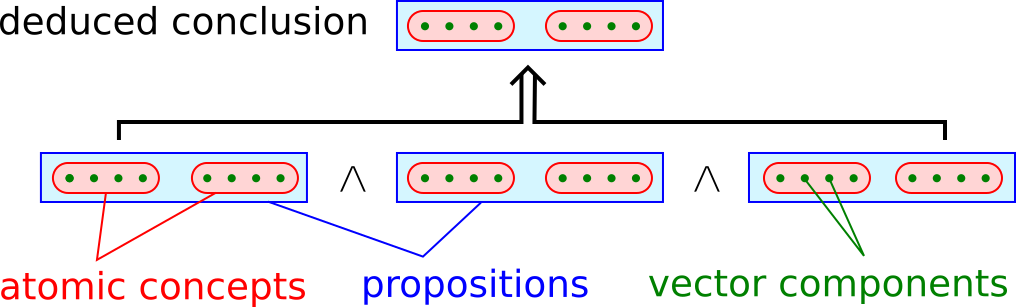
\includegraphics[scale=1]{logic-symmetry-predicate-level.png}}}
\end{equation}

\cc{相比之下,我们目前可以写出来的 代数关系 $p \wedge q = p \wedge q$ 只表达了这种结构:
}{
In contrast, the algebraic relation $p \wedge q = p \wedge q$ that we can currently write expresses only this structure:
}
\begin{equation}
\label{fig:logic-symmetry-propositional-only}
\vcenter{\hbox{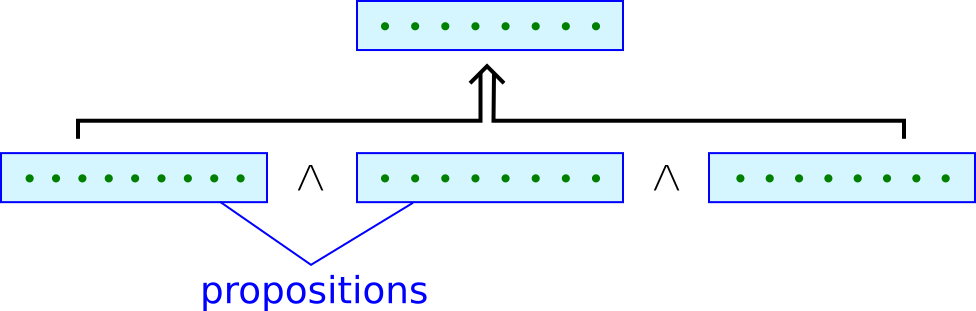
\includegraphics[scale=1]{logic-symmetry-propositional-only.png}}}
\end{equation}
\cc{相比于 图 (\ref{fig:logic-symmetry-propositional-only}),图 (\ref{fig:logic-symmetry-predicate-level}) 添加了 $\atom$ 的约束,\uline{但这约束怎样用代数表示}?
}{
Compared to figure (\ref{fig:logic-symmetry-propositional-only}), figure (\ref{fig:logic-symmetry-predicate-level}) adds $\atom$ constraints, \uline{but How can constraints be represented algebraically}?
}

\cc{而 \textbf{Transformer} 处理 命题 和 概念 的方式是这样:
}{
And the way \textbf{Transformer} handles propositions and concepts is this:
}
\begin{equation}
\label{fig:logic-symmetry-Transformer}
\vcenter{\hbox{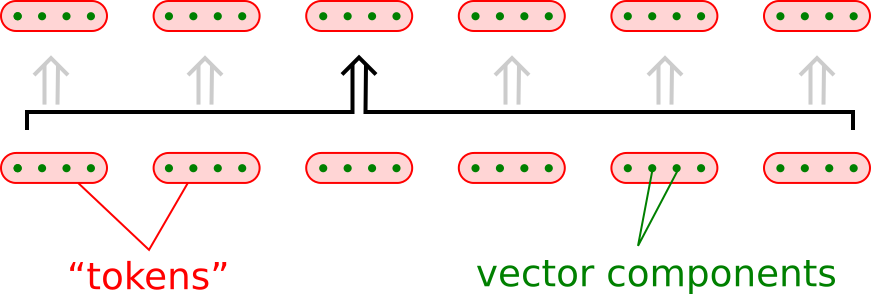
\includegraphics[scale=1]{logic-symmetry-Transformer.png}}}
\end{equation}
\cc{它没有 explicit 的命题结构,而是用特别的 token 表示句子的\textbf{终结},当然还有 positional encoding 这些「伎俩」。 所以,Transformer 是一种比较 \textit{ad hoc} 的设计,我们应该可以改进它。
}{
It does not have an explicit propositional structure, but uses a special token to represent the \textbf{end} of the sentence, and of course there are "tricks" such as positional encoding. So, Transformer is a rather \textit{ad hoc} design, and we should be able to improve it.
}

\end{minipage}
\end{preview}

\begin{preview}
\begin{minipage}{\textwidth}

\setlength{\parskip}{0.4\baselineskip}
\begin{textblock*}{20cm}(2.1cm,2cm) % {block width} (coords) 
	{\color{red}{\large \textcircled{\small 5}}}
	\hspace{8cm}
	\color{blue}{\footnotesize \cc{逻辑与深度学习}{Logic and Deep Learning}}
\end{textblock*}
\vspace*{0.3cm} 

\cc{现在我们企图回答那\uline{最重要的问题}: 怎样用代数形式表达「命题是由概念原子组成的」?
}{
Now we try to answer the \uline{the most important question}: how to express in algebraic form "a proposition is composed of conceptual atoms"?
}

\cc{亦即是说,以下这两个结构的分别在哪里? 如何用代数表达这不同?
}{
That is to say, what is the difference between the following two structures? How to express this difference algebraically?
}
\begin{equation}
\vcenter{\hbox{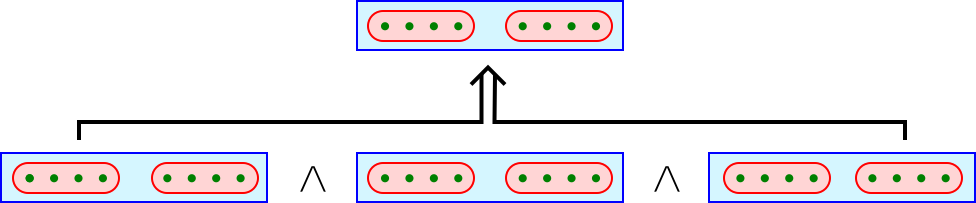
\includegraphics[scale=0.6]{logic-symmetry-predicate-level-1.png}}}
\quad \mbox{vs} \quad
\vcenter{\hbox{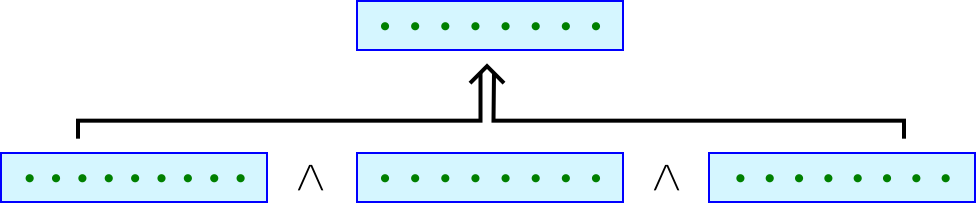
\includegraphics[scale=0.6]{logic-symmetry-propositional-only-1.png}}}
\end{equation}
\cc{这就像问 $ 0...9 \times 0...9 $ 跟 $ 00...99 $ 的分别(基本上没有分别,它们是 isomorphic)。 
}{
It's like asking $0...9 \times 0...9$ vs. $00...99$ (basically no difference, they're isomorphic).
}

\cc{类似地,
}{
Similarly,
}
\begin{equation}
\{ \mbox{ John, Mary } \} \times \{ \mbox{ human, god, worm } \}
\end{equation}
\cc{跟}{versus}
\begin{equation}
\{ \mbox{ John is human }, \mbox{ Mary is human }, .... \}
\end{equation}
\cc{等 $2 \times 3 = 6$ 个命题 也是同构的。 但前者是由两组不同的概念结合而成,它的成分可以被 $\forall$ 或 $\exists$ 量化; 后者是 命题逻辑,那些命题是不可分割的,也不可以拆开来量化。 
}{
These $2 \times 3 = 6$ propositions are also isomorphic. But the former is a combination of two different concepts, and its components can be quantified by $\forall$ or $\exists$; the latter is propositional logic, and those propositions are indivisible and cannot be separated and quantified.
}

\cc{但由于 $\atom \in$ 非交换自由群(最少结构的群),它没有像 $a \cdot b = b \cdot a$ 那样的对称性公式。
}{
But since $\atom \in$ is a non-commutative free group (the group with the least structure), it does not have a symmetry formula like $a \cdot b = b \cdot a$.
}

% 似乎要考虑  $\atom$ 的群结构是如何影响 逻辑 rule (\ref{fig:logic-symmetry-predicate-level}) 的输入和输出? 类似这样:
%\begin{equation}
%q_1 \cdot q_2 \; \Longleftarrow \; p_{11} \cdot p_{12} \; \wedge \; p_{21} \cdot p_{22}
%\end{equation}
%它跟这样有什么不同:
%\begin{equation}
%Q \; \Longleftarrow \; P_1 \; \wedge \; P_2 \quad ?
%\end{equation}

% $Q$ 是由两件东西组成,但这两件东西可以换成另外两件。 但那就不再是同一个 rule.  如果要维持是同一个 rule,则 任何 $\atom$ 元素不可以交换或更换。 那是不是需要考虑所有的 rules?

% 或者可以考虑一个 $\forall$ rule,它包含很多个 instantiated rules.  而它的 substitutions 总是以 群元素为 unit.  这一点可以怎样表示?

% 但其实当 rule 改变时,它似乎也是根据群元素的边界而改变的。 似乎一定要涉及大量的 rules 才可以表达 $\atom$ 的对称性。

% 但从机器学习的角度来看,rules 的更新 似乎没有必要 遵从 $\atom$ 的边界?

% 从经典 AI 的角度看,lattice of rules 结构 就是 algebra of atomic concepts 的结构。

% The proposition structure $P$ is made up of atoms $a$ from a free monoid $A$, and the rule can be quantified by $\forall$ and $\exists$ over such atoms.  ``The rule can be quantified'' means the mapping does not just send one compound element to another element, but that parts of the compound element can be varied and the output element would vary according to the rules of $\forall$ or $\exists$ as adjunctions to substitution maps.

% The \textbf{Atomic Condition} says that the input and output of a rule are made up of atoms that can vary according to $\forall$ and $\exists$ as adjoint functors.

% The \textbf{Atomic Condition} says that each $P_i = a_{i1} ... a_{ik}$ where some $a_{ij}$ \uline{can vary} according to $\forall$ and $\exists$ as adjoint functors.

% The \textbf{Atomic Condition} says that each $P_i = a_{i1} ... a_{ik}$ where some $a_{ij}$ \uline{can be copied} (possibly with some transformation) to another location.  And the transformation has to accord with $\forall$ and $\exists$ as adjunctions.

% The \textbf{Atomic Condition} says that each $P_i = a_{i1} ... a_{ik}$ where some $a_{ij}$ \uline{can be copied} (possibly with some transformation) to another location.  And the transformation has to accord with $\forall$ and $\exists$ as adjunctions.

% The \textbf{Atomic Condition} says that each $P_i = a_{i1} ... a_{iK}$ where some $a_{ih} = T_{\forall}(a_{jk})$ and the transformation $T_{\forall}$ has to accord with $\forall$ as an adjunction to a substitution functor.

\cc{经过一番分析之后 我得到了「命题是由概念原子构成的」以下条件:
}{
After some analysis I got the following condition for "propositions are made of conceptual atoms":
}

\begin{tcolorbox}[colback=white, enhanced]
\newtheorem*{condition}{Atomic Condition}
\begin{condition}[AC]
	Each proposition $P_i$ is made up of $K$ atoms:
	\begin{equation}
	P_i = a_{i1} \cdot ... \cdot a_{iK}
	\label{eqn:atomic-condition-1}
	\end{equation}
	where optionally some atoms can be \textbf{copied} to other locations (with a non-linear transformation $\tau$, if they are copied to the output layer) via:
	\begin{equation}
	a_{ih} = a_{jk} \quad \mbox{or} \quad a_{ih} = \tau(a_{jk})
	\label{eqn:atomic-condition-2}
	\end{equation}
	and the transformation $\tau$ has to accord with $\forall$ or $\exists$ as adjunctions to a substitution functor.
\end{condition}
\end{tcolorbox}

\cc{其实 $\tau$ 只需要是连续函数,就可以符合上述条件。 所以 Atomic Condition 的重点在于 (\ref{eqn:atomic-condition-1}) 和 (\ref{eqn:atomic-condition-2}) 这两个\textbf{等式},其实是非常简单的。 $\forall$ 和 $\exists$ 作为伴随函子 的范畴论描述 比较复杂,我们在 \hyperlink{page:appendix-A}{附录 A} 里解释。
}{
In fact, $\tau$ only needs to be a continuous function to meet the above conditions. So the focus of Atomic Condition lies in the two \textbf{equations} of (\ref{eqn:atomic-condition-1}) and (\ref{eqn:atomic-condition-2}), which are actually very simple. The category-theoretic description of $\forall$ and $\exists$ as adjoint functors is complicated, and we explain them in appendix {\color{red}{\large \textcircled{\small A}}}.
}

\cc{那么 等式 (\ref{eqn:atomic-condition-2}) 里面的 ``='' 是来自哪里? 其实太明显了,它就是逻辑 rule 里面 将变量「syntactically 搬动」的动作:
}{
So where does the ``='' in the equation (\ref{eqn:atomic-condition-2}) come from? In fact, it is too obvious, it is the action of "syntactically moving" the variable in the logic rule:
}
\vspace{0.5cm}
\begin{equation}
\forall X, Y, Z.  \;\;  \text{grandfather}({\color{red}X} \tikzmark{x}, {\color{red}Z} \tikzmark{z}) \leftarrow \text{father}({\color{red}X} \tikzmark{p}, {\color{red}Y} \tikzmark{y}) \wedge \mbox{father}({\color{red}Y} \tikzmark{q}, {\color{red}Z} \tikzmark{r})
\begin{tikzpicture}[overlay,remember picture,out=45,in=135,distance=1.1cm]
\draw[-,red, transform canvas={shift={(-5pt,18pt)}}] (x.center) to (p.center);
\draw[-,red, transform canvas={shift={(-5pt,18pt)}}] (y.center) to (q.center);
\draw[-,red, transform canvas={shift={(-5pt,-3pt)}}, out=-45,in=225] (z.center) to (r.center);
\end{tikzpicture}
\label{eqn:linkage-father}
\end{equation}
\cc{正是 这些「搬动」,构成了「命题是由概念组成的」结构。
}{
It is these "movements" that constitute the structure of "propositions are composed of concepts".
}

\end{minipage}
\end{preview}

\begin{preview}
\begin{minipage}{\textwidth}

\setlength{\parskip}{0.4\baselineskip}
\begin{textblock*}{20cm}(2.1cm,2cm) % {block width} (coords) 
	{\color{red}{\large \textcircled{\small 6}}}
	\hspace{8cm}
	\color{blue}{\footnotesize \cc{逻辑与深度学习}{Logic and Deep Learning}}
\end{textblock*}
\vspace*{0.3cm} 

\cc{\textbf{Self-Attention} 的本质 可以这样理解(抽象注意力结构):
}{
The essence of \textbf{Self-Attention} can be understood as follows (abstract attention structure):
}
\begin{equation}
\label{fig:abstract-self-attention}
\vcenter{\hbox{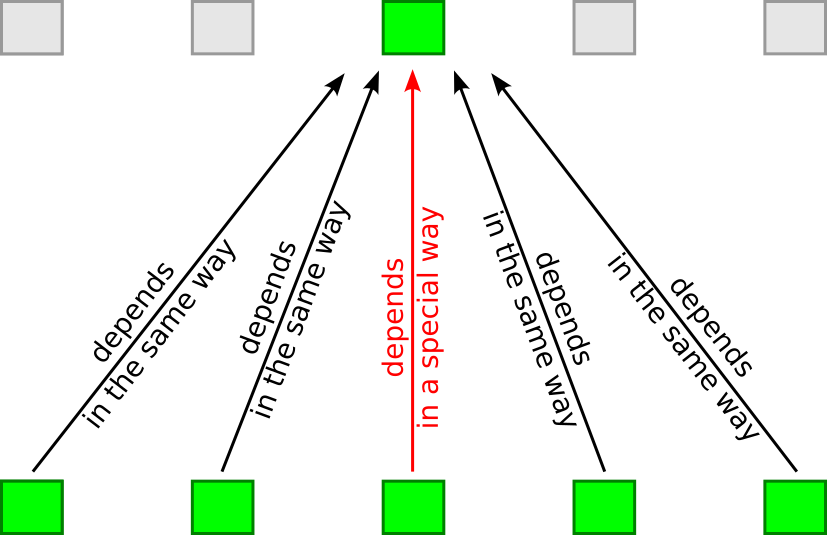
\includegraphics[scale=1]{essence-of-self-attention.png}}}
\end{equation}
\cc{这垂直的「軸」结构 ({\color{red}红色}),重复在每一条轴上。  所以,当 输入的元素 \textbf{交换}时,输出也随着交换。 这就是 self-Attention 能达到 \textbf{equi-variant} 效果的原因。
}{
This vertical "axis" structure ({\color{red}red}) is repeated on each axis. So, when the input elements are \textbf{swapped}, the output is also swapped. This is why self-Attention can achieve the \textbf{equi-variant} effect.
}

\cc{而我们想用 类似以上 self-Attention 的方法,解决 逻辑结构 的问题:
}{
And we want to use a method similar to the above self-Attention to solve the problem of logical structure:
}
\begin{equation}
\vcenter{\hbox{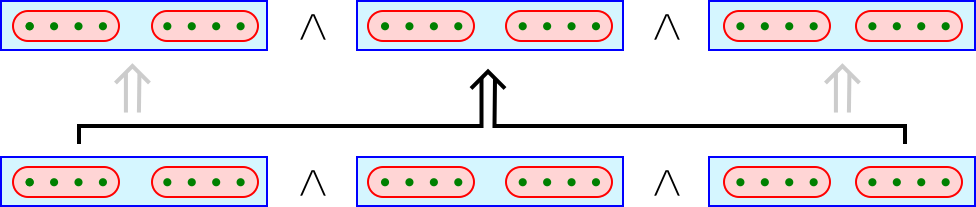
\includegraphics[scale=1]{logic-symmetry-logic-Transformer.png}}}
\end{equation}

\cc{这里有一个很重要的重点\footnote{谢谢 “子鱼” 告诉我这个重要信息。}: self-Attention 的前身是来自 Graves \textit{et al.} 的 《Neural Turing Machine》 的 \textbf{content-addressable memory}.  我们很有理由将它看成是一种 \textbf{记忆体}。
}{
Here is a very important point\footnote{Thank you "Ziyu" for telling me this important information. }: The predecessor of self-Attention is \textbf{content-addressable memory} from Graves \textit{et al.}'s "Neural Turing Machine". We have good reason to regard it as a kind of \textbf{memory} .
}

\cc{我们要比较 两种做法,前者是简单直接的经典 rule base 结构,后者是以 self-Attention 代替 rule base:
}{
We want to compare two approaches. The former is a simple and direct classic rule base structure, and the latter uses self-Attention instead of rule base:
}
\begin{equation}
\label{fig:rule-base}
\vcenter{\hbox{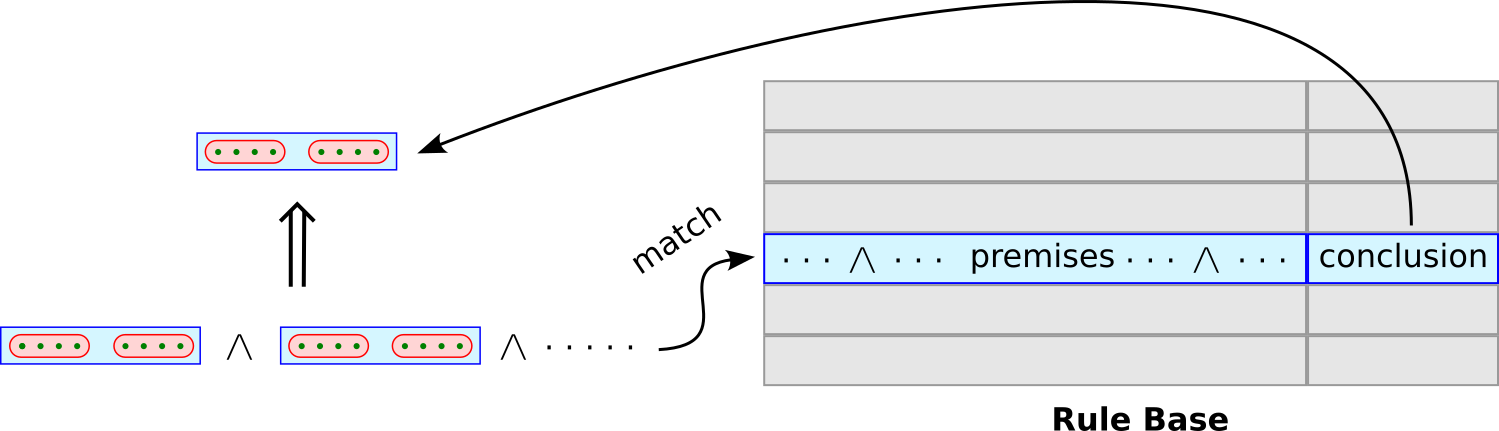
\includegraphics[scale=1]{shallow-rule-base.png}}}
\end{equation}
\hrule
\begin{equation}
\vcenter{\hbox{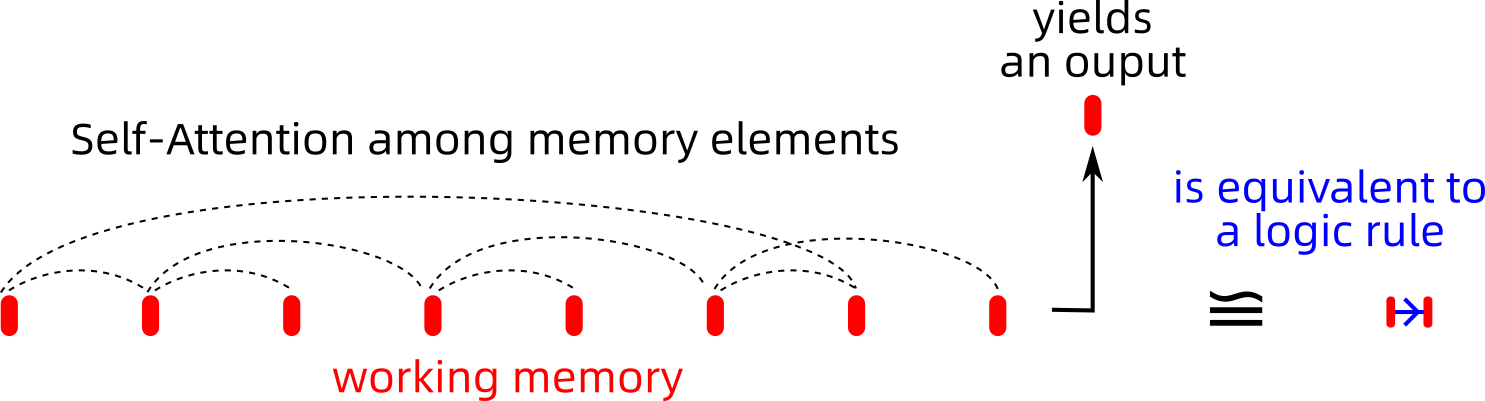
\includegraphics[scale=0.9]{rete-explained-3b.png}}}
\tag{\ref{fig:self-attention-as-Rete}}
\end{equation}
\cc{大家要感受到 Transformer 是一种非常 ``twisted'' 的处理 rules matching 的方式。 这个对应很不明显,以至于我们很难分辨出 Transformer 那边的 rules 长什么样子。 然而我觉得 Transformer 的设计者们 或许多少有意识到它跟 rule-based systems 的相似性。 特别地,看看以下这条逻辑 rule:
}{
Everyone should feel that Transformer is a very "twisted" way of dealing with rules matching. This correspondence is not obvious, so that it is difficult for us to tell what the rules on the Transformer side look like. However, I think the designers of Transformer may be somewhat aware of its similarity to rule-based systems. In particular, look at the following logical rule:
}
\vspace{0.5cm}
\begin{equation}
\forall X, Y, Z.  \;\;  \text{grandfather}(X \tikzmark{x1}, Z \tikzmark{z1}) \leftarrow \text{father}(X \tikzmark{x2}, {\color{red}Y} \tikzmark{y1}) \wedge \mbox{father}({\color{red}Y} \tikzmark{y2}, Z \tikzmark{z2})
\begin{tikzpicture}[overlay,remember picture,out=45,in=135,distance=1.1cm]
\draw[-, transform canvas={shift={(-5pt,18pt)}}] (x1.center) to (x2.center);
\draw[-,red, transform canvas={shift={(-5pt,18pt)}}] (y1.center) to (y2.center);
\draw[-, transform canvas={shift={(-5pt,-3pt)}}, out=-45,in=225] (z1.center) to (z2.center);
\end{tikzpicture}
\tag{\ref{eqn:linkage-father}}
\end{equation}
\cc{这 rule 的前提有两个条件,出现两次的变量 $Y$ 必须相等({\color{red}红色}),matching 才算成功。 而这种在 rule 的前提内部进行的 \textbf{比较} (comparison) 运作,正是 self-Attention 可以方便地做到的。 但 self-Attention 也忽略了 $A \wedge B$ 的对称性,可能还有改进的空间。
}{
The premise of this rule has two conditions, the variable $Y$ that appears twice must be equal ({\color{red}red}), and the matching is considered successful. And this kind of \textbf{comparison} operation inside the premise of the rule is exactly what self-Attention can do conveniently. But self-Attention also ignores the symmetry of $A \wedge B$, and there may be room for improvement.
}

\end{minipage}
\end{preview}

\begin{preview}
\begin{minipage}{\textwidth}

\setlength{\parskip}{0.4\baselineskip}
\begin{textblock*}{20cm}(2.1cm,2cm) % {block width} (coords) 
	{\color{red}{\large \textcircled{\small 7}}}
	\hspace{8cm}
	\color{blue}{\footnotesize \cc{逻辑与深度学习}{Logic and Deep Learning}}
\end{textblock*}
\vspace*{0.3cm} 

\cc{我觉得目前要回答的几个关键问题是:
}{
I think the key questions to be answered right now are:
}
\begin{itemize}
\cc{	\item 根据例如 刘乾 \textit{et al} 的论文\footnote{Qian Liu, Shengnan An, Jian-Guang Lou, Bei Chen, Zeqi Lin, Yan Gao, Bin Zhou, Nanning Zheng, and Dongmei Zhang. \textit{Compositional Generalization by Learning Analytical Expressions.} Advances in Neural Information Processing Systems 33 (2020).},Transformer 做不到某些 逻辑语法上的运作,问题出在哪里? 似乎不是 Transformer 根本无法学习那种语法,而是 它不能纯粹靠 prompt 做到。 但其实 prompt 是否具有深层意义,还是它只是一个 hack?  我们没有 explicitly「告诉」Transformer 它应该怎么做,那它做不到是不是一个真的缺憾? 我觉得很难判断,令 prompt 的研究方向笼罩在迷雾之中。
}{
\item According to e.g. Qian Liu's paper \footnote{Qian Liu, Shengnan An, Jian-Guang Lou, Bei Chen, Zeqi Lin, Yan Gao, Bin Zhou, Nanning Zheng, and Dongmei Zhang. \textit{ Compositional Generalization by Learning Analytical Expressions.} Advances in Neural Information Processing Systems 33 (2020).}, Transformer can't do some logical and grammatical operations, where is the problem? It doesn't seem like Transformer can't learn that syntax at all, but that it can't do it purely from prompts. But does prompt actually have a deeper meaning, or is it just a hack? We didn't explicitly "tell" the Transformer what it should do, so is it a real shortcoming that it can't do it? I find it difficult to judge, and the research direction of prompt is shrouded in fog.
}
	
\cc{	\item 现在考虑图 (\ref{fig:rule-base}) 即 rule base 的 na\"{i}ve 学习算法。 这个算法当然是很慢的,因为要比较两个集合(working memory 和 rule head)的相似性。 假设两个集合的大小固定为 $N$,那需要 $N \times N$ 次的 dot products,而这只是比较了一条 rule.  所有 rules 还要用 softmax 相加。 当 rule base 很大的时候,这个算法似乎不太实际。
}{
\item Now consider the na\"{i}ve learning algorithm for the graph (\ref{fig:rule-base}) that is the rule base. This algorithm is of course very slow, since two sets (working memory and rule head ) similarity. Assuming that the size of the two sets is fixed at $N$, then $N \times N$ times of dot products are needed, and this is just a comparison of a rule. All rules need to be added with softmax. When the rule base When it is very large, this algorithm seems impractical.
}
	
\cc{	\item 图 (\ref{fig:rule-base}) 还有可能出现 旧有的逻辑 rule learning 算法的问题,亦即 ``\textbf{plateau problem}''.  举例来说,用 Prolog 语言写 append 函数:\\
}{
\item figure (\ref{fig:rule-base}) may also have the problem of the old logic rule learning algorithm, that is ``\textbf{plateau problem}''. For example, write append in Prolog language function:\\
}
	\code{append(X,Y,Z) :-} \\
	\tab \code{list(X), head(X,X1), tail(X,X2), append(X2,Y,W), cons(X1,W,Z).} \\
\cc{	这个 rule 有 5个前提。 当 rule 被学习时,前提被逐个加进去,但 rule 的「得分值」一直是零,直到最后的前提 加进去了,得分才突然升到 100\%.  对于机器学习来说,这情况是很糟的。 而 Transformer 将 rules「扭曲地」缠在一起,这做法会不会反而有利于避免困在 local minima 呢?
}{
This rule has 5 premises. When the rule is learned, the premise is added one by one, but the "score value" of the rule is always zero, until the last premise is added, the score suddenly rises to 100\%. For machine learning, this situation is Terrible. And the Transformer twists the rules together. Will this approach help avoid being trapped in the local minima?
}
	
\cc{	\item 可能存在 介乎 Transformer 与 na\"{i}ve rule base 之间的算法,它比 Transformer 有更强的逻辑结构,但比 na\"{i}ve rule base 用了更多类似 self-Attention 的矩阵运算来加速?
}{
	\item May have an algorithm between Transformer and na\"{i}ve rule base, it has a stronger logical structure than Transformer, but uses more similar self-Attention's matrix operation to speed up?
}
\end{itemize}

\end{minipage}
\end{preview}

\begin{preview}
\begin{minipage}{\textwidth}

\setlength{\parskip}{0.4\baselineskip}
\begin{textblock*}{20cm}(2.1cm,2cm) % {block width} (coords) 
	{\color{red}{\large \textcircled{\small 8}}}
	\hspace{8cm}
	\color{blue}{\footnotesize \cc{逻辑与深度学习}{Logic and Deep Learning}}
\end{textblock*}
\vspace*{0.3cm} 

\cc{现时想到的一个比较可行的 architecture:
}{
A more feasible architecture that I think of now:
}
\begin{equation}
\cc{  \vcenter{\hbox{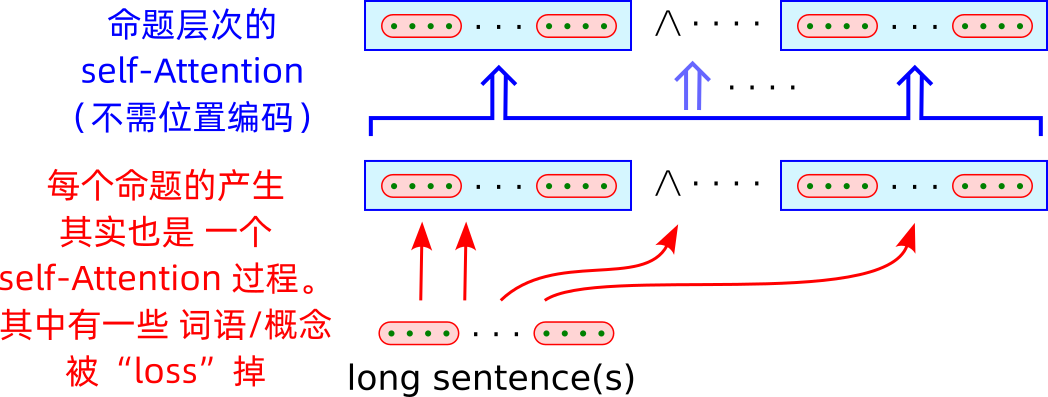
\includegraphics[scale=1]{seq-to-seq-seq-with-Transformer.png}}}      }{
      \vcenter{\hbox{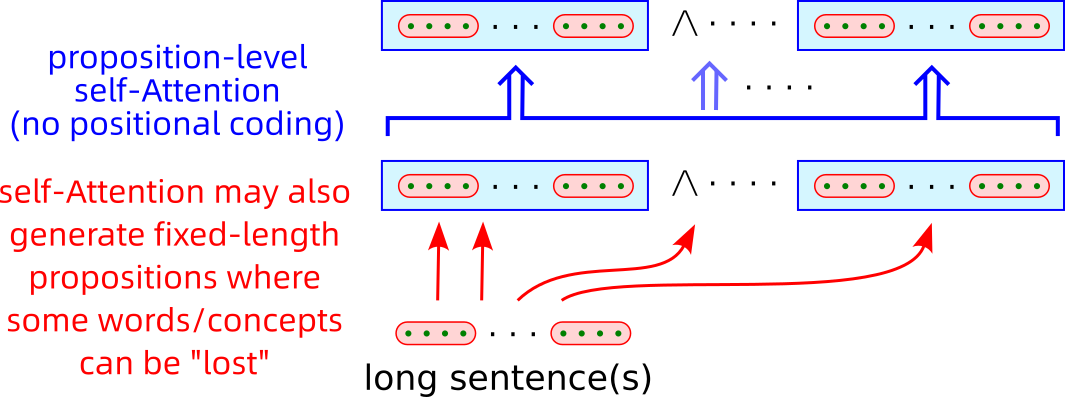
\includegraphics[scale=1]{seq-to-seq-seq-with-Transformer-en.png}}}   }
\end{equation}
\begin{itemize}
\cc{	\item 在{\color{blue}蓝色}结构里,每个命题要由 fixed \# of 概念原子组成。
}{
\item In the {\color{blue}blue} structure, each proposition shall consist of fixed \# of concept atoms.
}

\cc{	\item 但抽象的 self-Attention 结构也可以容许 \textbf{可变长度} 的命题,只要能计算到 命题之间的 \textbf{dot product} (similarity) ,还有 读取 固定长度的 \textbf{矩阵} 记忆体。
}{
\item But the abstract self-Attention structure can also allow \textbf{variable length} propositions, as long as the \textbf{dot product} (similarity) between the propositions can be calculated, and the fixed-length \textbf{ matrix} memory.
}

\cc{	\item {\color{red}红色}结构: 如何从 不定长度的句子 产生数量和长度不同的命题? 这就是以前谈过的 sequence to sequence-of-sequences 问题。 这也可以用 ``lossy'' self-Attention 解决。
}{
\item {\color{red}red} structure: how to generate propositions of varying number and length from sentences of indefinite length? This is the sequence to sequence-of-sequences problem discussed before. This can also be solved with ``lossy'' self-Attention.
}
	
\end{itemize}

\end{minipage}
\end{preview}

\begin{preview}
\begin{minipage}{\textwidth}
\hypertarget{page:appendix-A}{}

\setlength{\parskip}{0.4\baselineskip}
\begin{textblock*}{20cm}(2.1cm,2cm) % {block width} (coords) 
	{\color{red}{\large \textcircled{\small A}}}
	\hspace{8cm}
	\color{blue}{\footnotesize \cc{逻辑与深度学习}{Logic and Deep Learning}}
\end{textblock*}
\vspace*{0.3cm} 

在这个附录里,我们用简单的方式解释一下 $\forall$ 和 $\exists$ 的理论。 

以下是一个关系 $R$,例如「$Y$爱$X$」,$X, Y$ 都是「人」的集合;两个相同的拷贝。 例如 对角线 代表爱自己(有些人不爱自己)。 注意这个图也不是 对角线 对称的,否则就没有「失恋」了。 将关系 $R$ 的图像 \textbf{投影} 到 $X$ 轴上,可以得到 $\forall_Y$ 和 $\exists_Y$ 集合。 $\forall_Y$ 集合 代表那些「人人都爱」的 $X$,$\exists_Y$ 集合代表那些「有人爱他」的 $X$:
\begin{equation}
\vcenter{\hbox{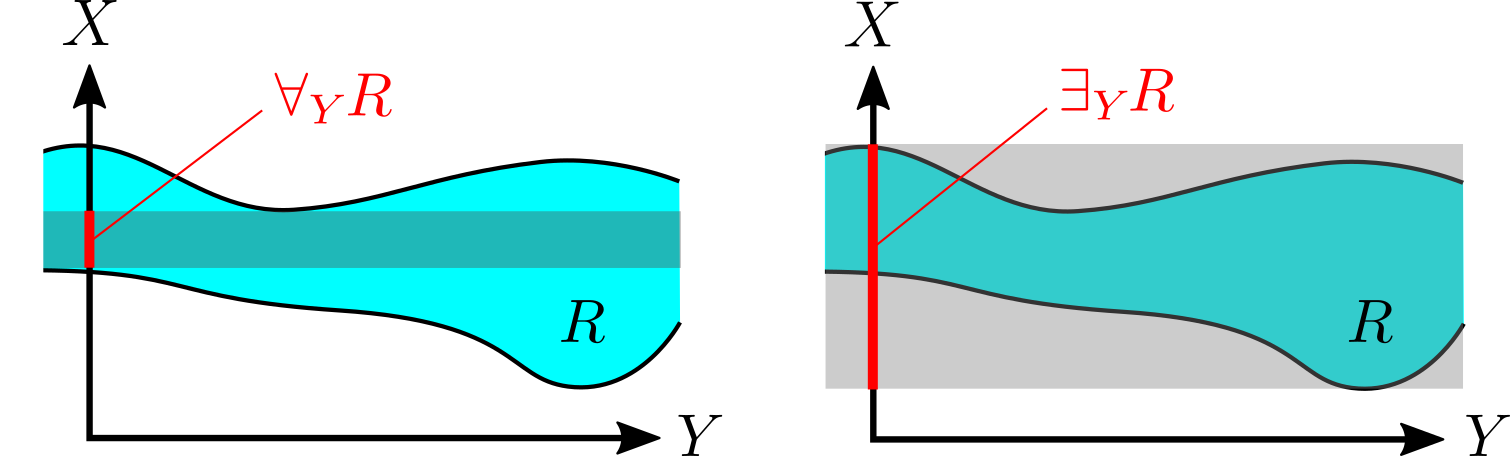
\includegraphics[scale=0.8]{forall-and-exists.png}}}
\end{equation}
范畴论大师 Lawvere 发现,$\forall$ 和 $\exists$ 是一个所谓 \textbf{weakening functor} 的「伴随函子」,所谓 weakening 就是从一个只有 $X$ 变量的\textbf{论域} 扩充到有 $X,Y$ 两个变量的论域,而这里 $Y$ 纯粹是一个 \textbf{dummy} variable:
\begin{equation}
\begin{tikzcd}[column sep = 4cm, row sep = 0.3cm]
{}  & {} \arrow[l, swap, "\forall_Y"] \\
(X) \arrow[r, "\mbox{weakening}"] & (X,Y) \\
{}  & {} \arrow[l, swap, "\exists_Y"]
\end{tikzcd}
\end{equation}
例如 $\mbox{Love}(Y,X)$ 是带有两个变量的逻辑式子,但 $\forall Y. \mbox{ Love}(Y,X)$ 其实没有了 $Y$ 这个变量,因为它被 $\forall$ \textbf{绑定}了。

所谓 \textbf{伴随} (adjoint) 的意思是: 有两个范畴:左边和右边。 你可以将 左边的东西搬到右边,在右边的范畴里做「\textbf{比较}」,而这个比较 同样地可以 把东西搬到左边做,两个比较是\textbf{等价}的。 这里「比较」的意思就是范畴内的 morphism, 例如在 $\mathsf{Set}$ 范畴里,比较就是 set inclusion.  

伴随函子 并不是唯一的,所以 weakening 分别有 $\forall$ 和 $\exists$ 两个伴随。

\cc{Lawvere 将 量词 $\forall$ 和 $\exists$ 推广得更一般: 「简单」的 weakening functor 是基于 笛卡尔积 $X \times Y$; Lawvere 将它扩充到任何 \textbf{substitution} functor.  但我暂时缺乏这方面的例子,不清楚它对我们的应用有什么益处。
}{
	Lawvere's work made the $\forall$ and $\exists$ quantifiers more general: the ``simple'' weakening functor is based on the Cartesian product $X \times Y$, but Lawvere expanded it to arbitrary \textbf{substitution} functors.  (I don't know of examples of this, so I'm not sure what advantages this could bring to our application.)
}

\end{minipage}
\end{preview}

\begin{preview}
\begin{minipage}{\textwidth}

\setlength{\parskip}{0.4\baselineskip}
\begin{textblock*}{20cm}(2.1cm,2cm) % {block width} (coords) 
	{\color{red}{\large \textcircled{\small B}}}
	\hspace{8cm}
	\color{blue}{\footnotesize \cc{逻辑与深度学习}{Logic and Deep Learning}}
\end{textblock*}
\vspace*{0.3cm} 

%我们希望 以代数形式表达 谓词 $\atom$ 的颗粒性。 
\cc{在 范畴逻辑 里面有 \textbf{Beck-Chevalley} 条件和 \textbf{Frobenius} 条件,或许是我们所需的对称性? 但细看之后,发觉还是不能解决问题.....  For completeness,我还是描述一下,没兴趣的可以略过。
}{
In categorical logic there are \textbf{Beck-Chevalley} conditions and \textbf{Frobenius} conditions, perhaps the symmetry we need? But after a closer look, I found that the problem still cannot be solved... For completeness, I will describe it, and you can skip it if you are not interested.
}

\cc{首先考虑比较容易明白的 \textbf{Frobenius} 条件。 在逻辑上,它等于说:
}{
Consider first the easier-to-understand \textbf{Frobenius} condition. Logically, it is equivalent to saying:
}
\begin{equation}
\exists x. [ \phi \wedge \psi(x) ] \equiv \phi \wedge \exists x. \psi(x).
\end{equation}
\cc{由于 经典逻辑 AI 普遍使用 $\forall$ 而忽略 $\exists$,我将上式改写成:
}{
Since classical logic AI generally uses $\forall$ and ignores $\exists$, I rewrite the above formula as:
}
\begin{equation}
\label{eqn:Frobenius-condition}
\forall x. [ \phi \vee \psi(x) ] \equiv \phi \vee \forall x. \psi(x).
\end{equation}
\cc{但问题是,(\ref{eqn:Frobenius-condition}) 式的左边和右边,其对应的神经网络 (\ref{fig:logic-symmetry-predicate-level}) 是一样的(看不出有分别)。 也就是说这个差别可能太 subtle 了,它并不影响我们实际 implement 的神经网络。
}{
But the problem is, the left and right sides of the formula (\ref{eqn:Frobenius-condition}), the corresponding neural network (\ref{fig:logic-symmetry-predicate-level}) is the same (no difference ). In other words, this difference may be too subtle, and it does not affect the neural network we actually implement.
}

%\cc{在逻辑里,任何变量 例如 $x,y$ 等,必须被 $\forall$ 或 $\exists$ quantify,否则不成为合法的句子。 所以 表达 谓词结构的对称性,也很可能要涉及 $\forall$ 或 $\exists$.
%}{
%In logic, any variable such as $x, y$, etc. must be quantified by $\forall$ or $\exists$, otherwise it will not become a legal sentence. So to express the symmetry of the predicate structure, it is also likely to involve $\forall$ or $\exists$.
%}

\end{minipage}
\end{preview}

\begin{preview}
\begin{minipage}{\textwidth}
		
\setlength{\parskip}{0.4\baselineskip}
\begin{textblock*}{20cm}(2.1cm,2cm) % {block width} (coords) 
	{\color{red}{\large \textcircled{\small C}}}
	\hspace{8cm}
	\color{blue}{\footnotesize \cc{逻辑与深度学习}{Logic and Deep Learning}}
\end{textblock*}
\vspace*{0.3cm} 

\cc{以前说过,谓词逻辑 带来 \textbf{fibration} 或 \textbf{indexing} 结构。 Beck-Chevalley 和 Frobenius 条件 基本上是说,这 纤维结构 是 ``preserved by re-indexing functors''.
}{
As said before, predicate logic leads to \textbf{fibration} or \textbf{indexing} constructs. The Beck-Chevalley and Frobenius conditions basically say that the fiber structure is ``preserved by re-indexing functors''.
}

\cc{这是 fibration 结构的示意图:
}{
Here is a diagram of the fibration structure:
}
\begin{equation}
\vcenter{\hbox{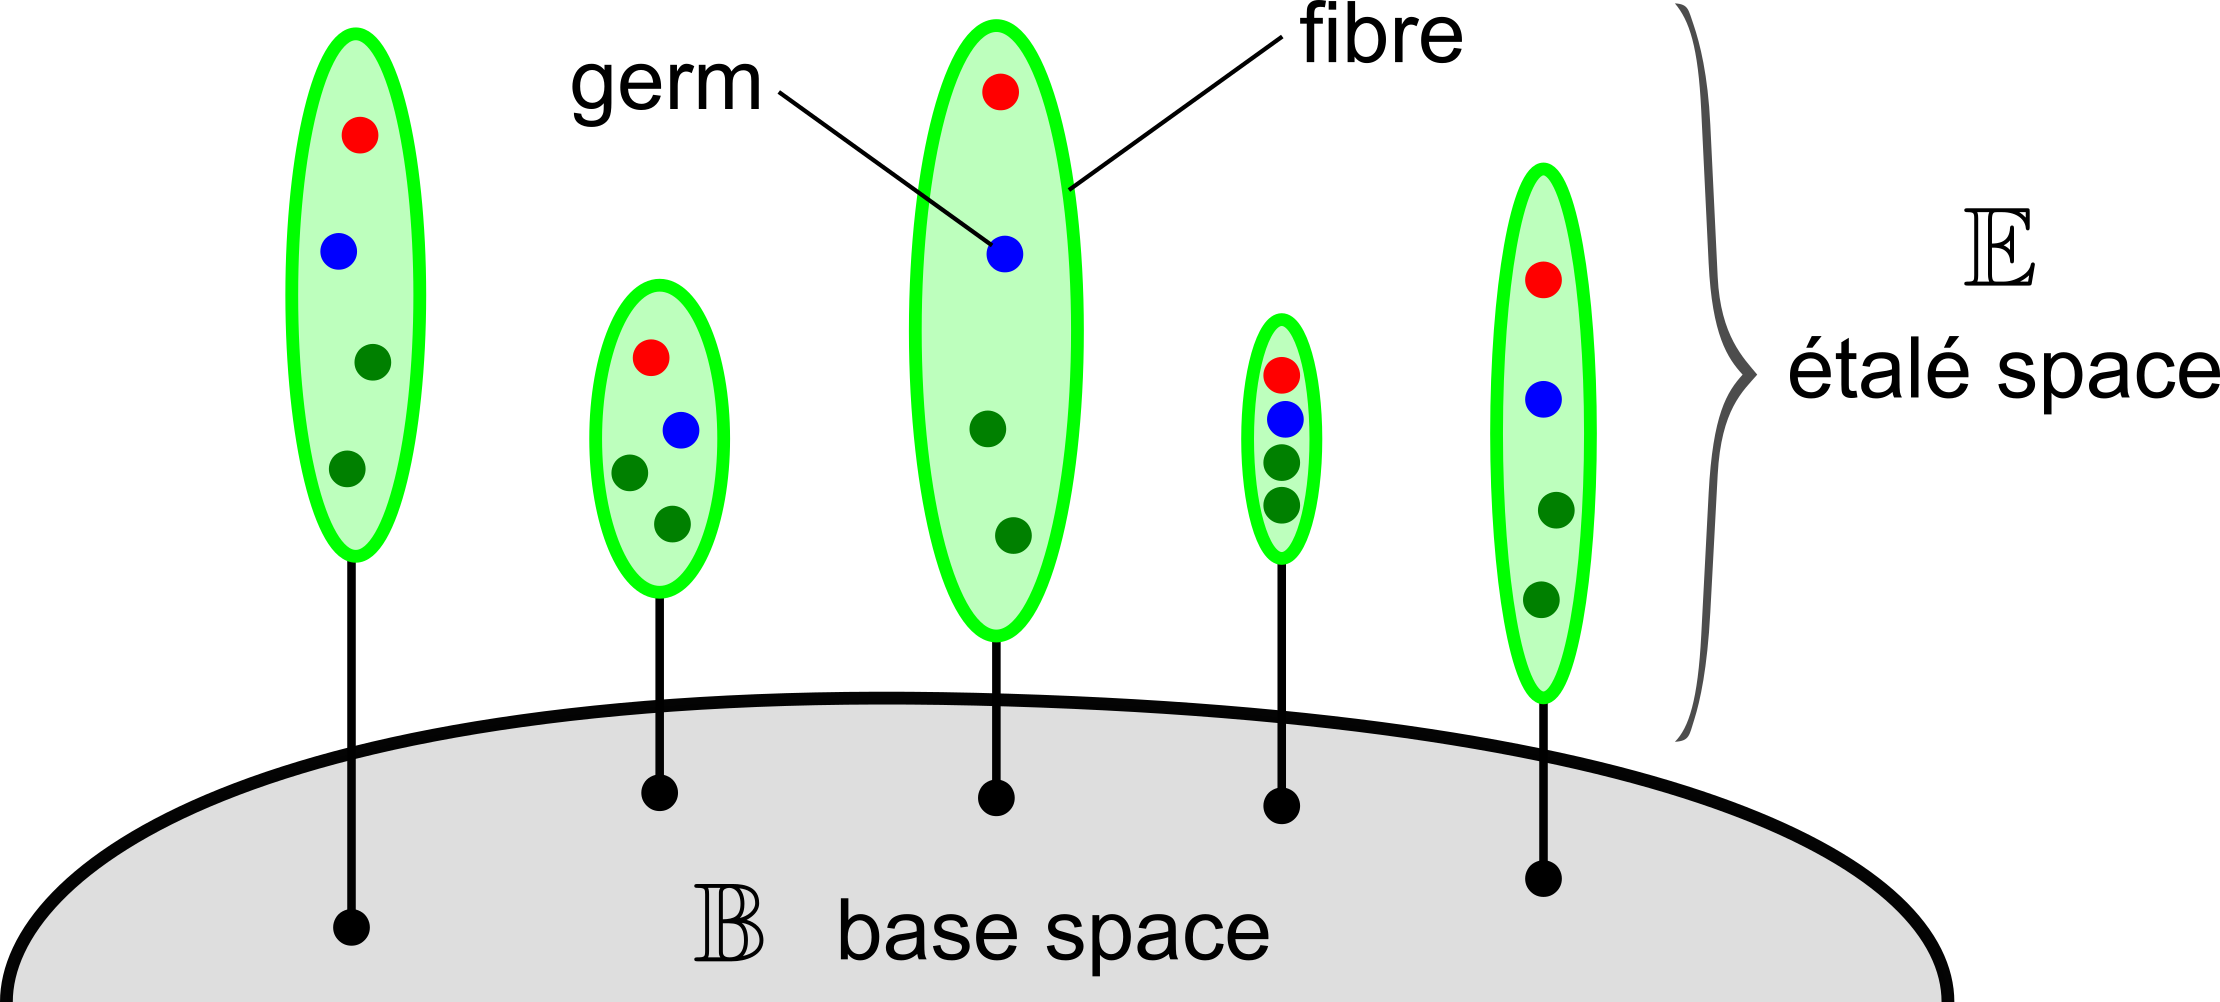
\includegraphics[scale=0.7]{etale-space.png}}}
\end{equation}
\cc{这整个结构 叫 \textbf{bundle},而 \textbf{sheaf} 是 bundle 加上某个特殊的 拓扑结构。 
}{
This whole structure is called \textbf{bundle}, and \textbf{sheaf} is bundle plus some special topology.
}

\cc{在 $(A,f)$ 和 $(B,g)$ 两个 bundle 之上可以定义 \textbf{fibred product} of $A$ and $B$ over $I$, 记作 $A \times_I B$:
}{
\textbf{fibred product} of $A$ and $B$ over $I$ can be defined on top of the two bundles $(A,f)$ and $(B,g)$, denoted as $A \times_I B$ :
}
\begin{equation}
\label{eqn:fibred-product}
\begin{tikzcd}[sep = 3cm]
A \times B \arrow[r, "q"] \arrow[d, swap, "p"] \arrow[rd, "h"] & B \arrow[d, "g"] \\
A \arrow[r, swap, "f"] & I
\end{tikzcd}
\end{equation}
\cc{其中 $h = f \circ p = g \circ q$.  这也是一个 \textbf{pullback}.
}{
where $h = f \circ p = g \circ q$. This is also a \textbf{pullback}.
}

\cc{\textbf{Beck-Chevalley} 条件是说 下面这幅图 commute: 
}{
The \textbf{Beck-Chevalley} condition says that the following image commute:
}
\begin{equation}
\label{eqn:Beck-Chevalley}
\begin{tikzcd}[column sep = 3cm]
K \times J \arrow[r, "u \;\times\; id"] \arrow[d, swap, "\pi"] & I \times J \arrow[d, "\pi"] \\
K \arrow[r, swap, "u"] & I
\end{tikzcd}
\end{equation}
\cc{其中 $\pi$ 就是代表 量词 $\forall$ 或 $\exists$ 的 投影,它们是 weakening map $\pi^*$ 的伴随映射。 
}{
where $\pi$ is the projection representing the quantifier $\forall$ or $\exists$, which are the accompanying maps of the weakening map $\pi^*$.
}

\cc{Beck-Chevalley 条件并不完全是空洞的;它有可能不成立。 有一个反例是 Pitts 提出的: 考虑 $X \times Y$, 其中 $X = Y = \mathbb{N} \cup \{\infty\}$ 亦即 自然数加上 $\infty$ 作为 top element; 但 $Y$ 是用 discrete order,亦即所有 order 都是 = 关系。  $A$ 是 $X \times Y$ 上的关系: $A = \{ (x,y) \in \mathbb{N \times N} \;|\; x \le y \}$.  那么 $\exists y. (x,y) \in A$ 会是整个 $X$ 集合。 如果考虑 DCPO 范畴,我们要求 fibration of Scott-closed subsets (ordered by inclusion) over DCPO.  $\exists y. A$ 的 Scott closure 的条件是 它是一个 lower set closed under directed joins; 而这个 Scott closure 条件似乎不成立,因而导致 图 (\ref{eqn:Beck-Chevalley}) 不 commute.(我对 Scott closure 的细节不太理解)
}{
The Beck-Chevalley condition is not entirely hollow; it may not hold. There is a counter-example from Pitts: Consider $X \times Y$, where $X = Y = \mathbb{N} \cup \{\infty\}$ is the natural number plus $\infty$ as top element; but $Y$ uses discrete order, that is, all orders are = order. $A$ is the relationship on $X \times Y$: $A = \{ (x,y) \in \mathbb{N \times N} \;|\; x \le y \}$. Then $\exists y. (x,y) \in A$ will be the entire set of $X$. If we consider the DCPO category, we require the fibration of Scott-closed subsets (ordered by inclusion) over DCPO. The condition for Scott closure of $\exists y. A$ is that it is a lower set closed under directed joins; and this Scott closure condition seems to be violated, thus causing the graph (\ref{eqn:Beck-Chevalley}) not to commute. (I do not understand the details of Scott closure)
}

\end{minipage}
\end{preview}

\begin{preview}
	\begin{minipage}{\textwidth}
		
		\color{teal}
		
\cc{首先以函数的方式表达 self-Attention 结构:
}{
	First express the self-Attention structure in a functional way:
}
\begin{eqnarray}
\cc{
	\boxed{\mbox{输出命题 $O_i$ 由原子 $b_i$ 组成}} \quad O_i &=& [b_1 ... b_K] \\
	\boxed{\mbox{输入命题 $P_i$ 由原子 $a_i$ 组成}} \quad P_i &=& [a_1 ... a_K] \\
}{
	\boxed{\mbox{output proposition $O_i$ is composed of atoms $b_i$ }} \quad O_i &=& [b_1 ... b_K] \\
	\boxed{\mbox{input proposition $P_i$ is composed of atoms $a_i$ }} \quad P_i &=& [a_1 ... a_K] \\
}
\boxed{\mbox{Self-Attention}} \quad O_i = \alpha(P_i \;; P_1 ... \hat{P_i} ... P_N)
\end{eqnarray}
\cc{$P_1 ... \hat{P_i} ... P_N$ 的意思是 $P_1 ... P_N$ 除了 $P_i$. \\
}{
	$P_1 ... \hat{P_i} ... P_N$ means $P_1 ... P_N$ except $P_i$. \\
}
\cc{$\alpha(P_i \;; ... )$ 是图 (\ref{fig:abstract-self-attention}) 的函数结构,也可以理解为 以 $P_i$ 为 query 的 self Attention.
}{
	$\alpha(P_i \;; ... )$ is the function structure of the graph (\ref{fig:abstract-self-attention}), and it can also be understood as the self Attention with $P_i$ as the query.
}

		How to measure similarity between $(P_i, Q_i)$?
		\begin{equation}
		\argmin_i \sum_i \min_j \langle P_i, Q_j \rangle
		\end{equation}
		
		\begin{itemize}
			\cc{	\item 首先留意到,轴心结构 只对 命题层次有用,它的作用不会延伸到 概念原子层次。 然而,有监于 Transformer 也没有充分利用 交换不变性,然而它却因为用了矩阵乘法而变得很有效率,所以从效率的角度看,也有将 轴心结构 延伸到 原子层面的理由。
			}{
				\item First notice that the pivot structure is only useful at the propositional level, and its effect does not extend to the conceptual atomic level. However, since Transformer does not take full advantage of the exchange invariance, it becomes very efficient because it uses matrix multiplication, so from an efficiency point of view, there are also reasons to extend the axis structure to the atomic level.
			}
			
			\cc{	\item 另一个可以尝试的想法是: 直接 hard-code copying mechanism.  这可以怎样用 Attention 做到?  以前分析过了,copy 并不容易,因为需要 winner takes all.
			}{
				\item Another idea to try is: direct hard-code copying mechanism. How can this be done with Attention? It has been analyzed before, copy is not easy, because winner takes all.
			}
			
			\cc{	\item 但纯粹用 Hopfield network 又缺乏了 深度。 但似乎 在 RL 场景下,\textbf{广度} 也是重要的。
			}{
				\item but purely using Hopfield network lacks depth. But it seems that in the RL scenario, \textbf{breadth} is also important.
			}
			
			\cc{	\item 其实 只要有 输入/输出 的函数关系,就等价于有 逻辑 rules 的 KB 库。 问题是它用什么方法给出结论。
			}{
				In fact, as long as there is an input/output functional relationship, \item is equivalent to a KB library with logic rules. The question is what method it uses to reach its conclusions.
			}
		\end{itemize}
		
		\cc{Self-Attention 已经符合我们的要求,但我们想改进它。 主要有两个 idea: 其一是更直接的 copy mechanism,其二是 更细致的 函数 dependence.
		}{
			Self-Attention already meets our requirements, but we want to improve it. There are two main ideas: one is a more direct copy mechanism, and the other is a more detailed function dependency.
		}
		\begin{equation}
		\vcenter{\hbox{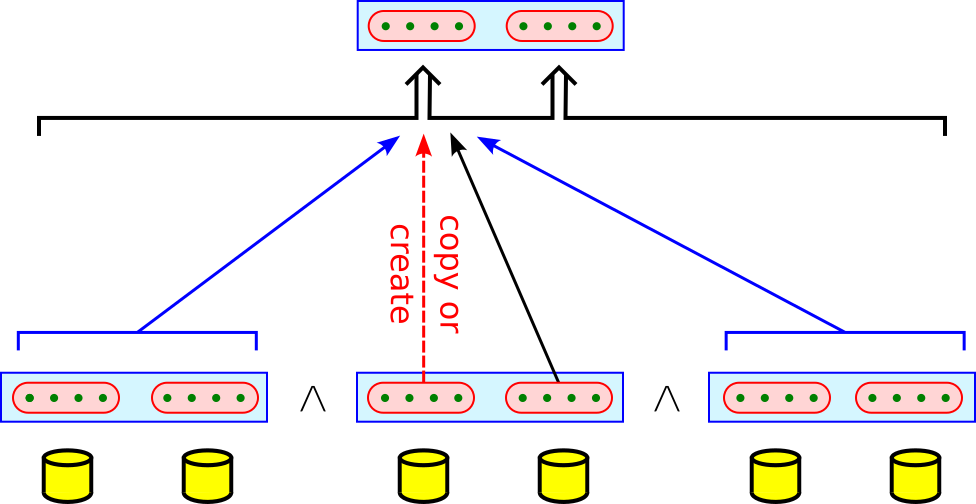
\includegraphics[scale=1]{logic-Transformer-1.png}}}
		\end{equation}
		
		\textbf{Copy:}
		\begin{itemize}
			\cc{	\item Copy 不需要什么特别机制,输出就是输入。 但问题是怎样 combine with ``create'' operation.
			}{
				\item Copy requires no special mechanism, the output is the input. But the question is how to combine with ``create'' operation.
			}
			\cc{	\item 当然 可以用大家都熟悉的 softmax: $ \alpha \mbox{ copy} + \beta \mbox{ create} $, where $\alpha, \beta$ are outputs of softmax.
			}{
				\item can of course use the familiar softmax: $ \alpha \mbox{ copy} + \beta \mbox{ create} $, where $\alpha, \beta$ are outputs of softmax.
			}
			\cc{	\item 另一个想法是 content-addressable.  用 table-lookup 的形式,找可执行的 rules。 但有 variable matching 的问题。 
			}{
				\item Another idea is content-addressable. Use table-lookup to find executable rules. But there is a problem with variable matching.
			}
		\end{itemize}
		
		\textbf{Create:}
		\begin{itemize}
			\cc{	\item 需要的是怎样的函数?
			}{
				\item What kind of function is needed?
			}
		\end{itemize}
		
	\end{minipage}
\end{preview}

\end{document}
